\documentclass[12pt]{article}

\usepackage[utf8]{inputenc}
%\usepackage{colortbl}
\usepackage[italian]{babel}
\usepackage{graphics,graphicx}
\graphicspath{{figs/}}
%\usepackage{algorithmic}
\usepackage[usenames,dvipsnames]{color}
\usepackage{pxfonts} % use pxfont
\usepackage{listings}
\usepackage{fancyvrb}

\title{\textbf{ASTRO} lib and Matlab Wrapper}
\author{Enrico Bertolazzi and Francesco Biral} %  Marco Galvani, Fabrizio Zendri
\date{1 August 2021}			

%%
\newcommand\codeHighlight[1]{\textcolor{Blue}{\textbf{#1}}}
\newcommand\method[1]{\textcolor{Orange}{#1}}
\newcommand\class[1]{\textcolor{NavyBlue}{\textbf{#1}}}
\newcommand{\HRule}{\rule{\linewidth}{0.1mm}}

%%
\begin{document}
\maketitle						


\section{\textbf{ASTRO} library}

\begin{figure}[h!]
	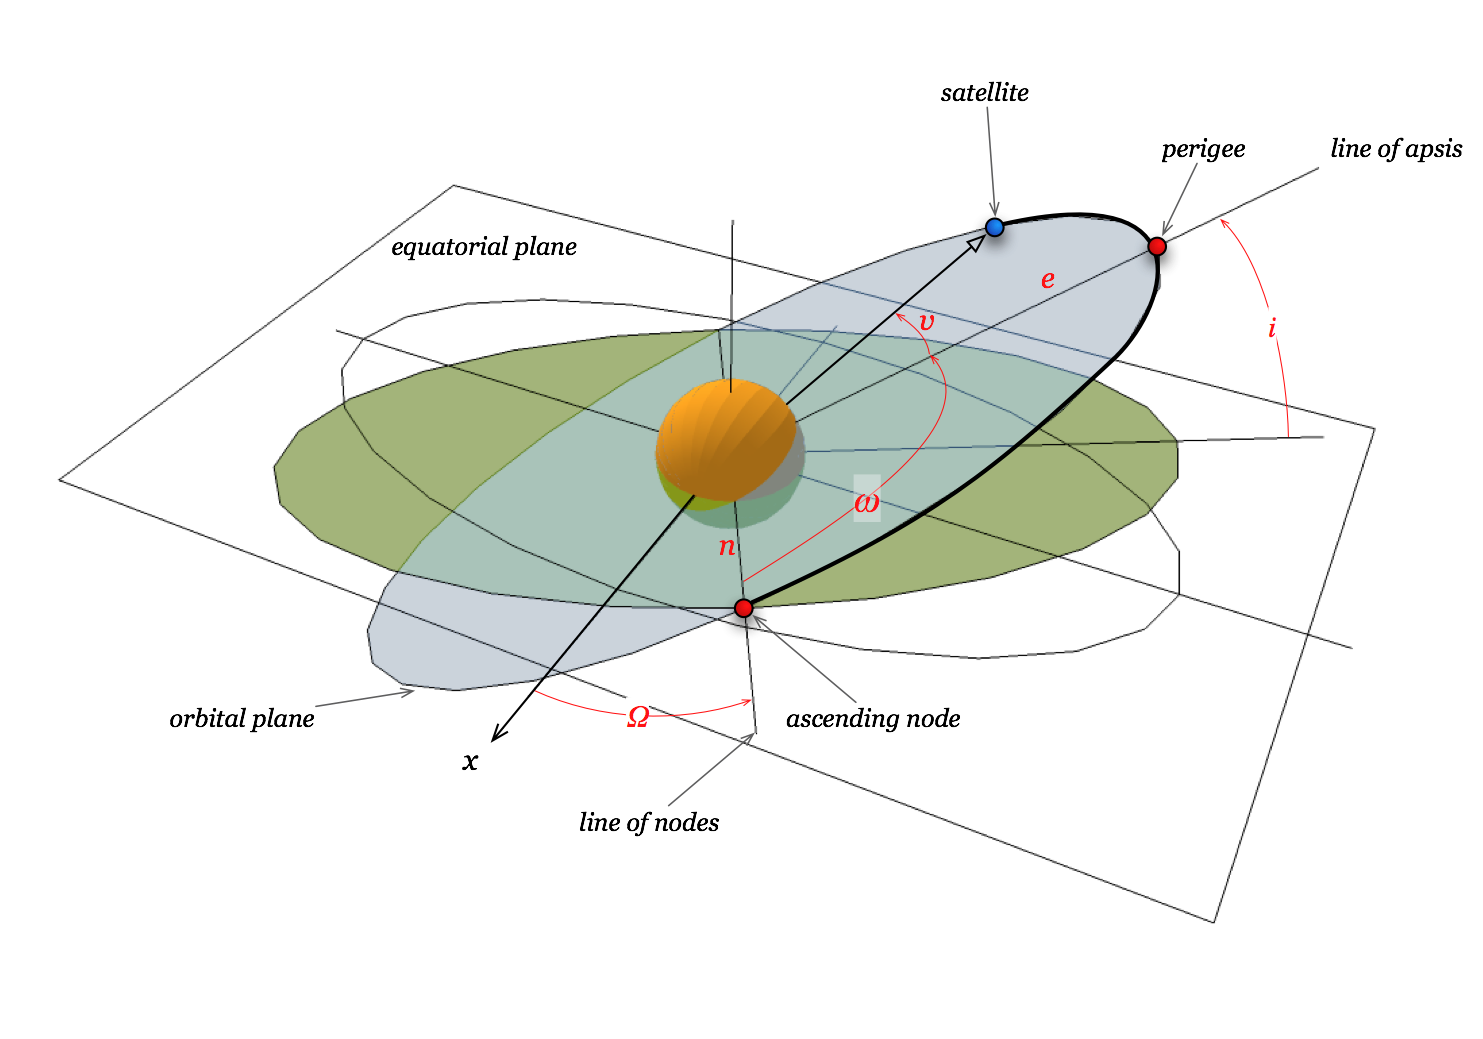
\includegraphics[width=1.0\textwidth]{coordinates}
\end{figure}


An astronomical unit (abbreviated as \textbf{AU}, \textbf{au}) is a unit of length equal to about 149,597,871 kilometres (92,955,807 miles) or approximately the mean EarthSun distance.

Il wrapper Matlab della libreria {\tt \textbf{\textbf{ASTRO}}} prevede un'unica chiamata in cui il primo argomento e' una stringa che specifica il metodo della libreria C++ da usare:
\\
\\
\\
I metodi resi disponibili dalla libreria \textbf{\textbf{ASTRO}} sono i seguenti: 
\\
\\
{\tt \class{ASTRO}(\method{'load'}, 'filename.txt')}\\
Carica il file dati degli asteroidi definiti con i parametri orbitali dal file {\tt 'filename.txt'}. Il file da caricare non è più la versione ``new'', ma quella originale.
\\
\HRule
\\
{\tt astName = \class{ASTRO}(\method{'getname'}, astNum)}\\
\\Restituisce il nome {\tt astName} dell'asteroide {\tt astNum}.
\\
\HRule
\\
{\tt year = \class{ASTRO}(\method{'period'}, astNum)}\\
\\Restituisce la durata dell'anno in giorni {\tt year} per l'asteroide {\tt astNum}.
\\
\HRule
\\
{\tt L = \class{ASTRO}(\method{'angle'}, astNum,t)}\\
\\Restituisce l'angolo {\tt L} in coordinate equinoziali dell'asteroide {\tt astNum} al tempo {\tt t} espresso in giorni. In questo caso, {\tt t} è un singolo istante e non un vettore di tempi.
\\
\HRule
\\
{\tt [e, a, i, Omega, omega] = \class{ASTRO}(\method{'orbitalclassic'}, astNum)}\\
\\Estrae i parametri orbitali classici (Kepleriani) dato il numero {\tt astNum} dell'asteroide. Si suppone di aver caricato nella memoria della libreria \textbf{\textbf{ASTRO}} i dati degli asteroidi.
\\
\HRule
\\
{\tt [p, f, g, h, k ] = \class{ASTRO}(\method{'orbitalequinoctial'}, astNum)}\\
\\Fornisce i parametri orbitali in coordinate equinoziali dell'asteroide numero {\tt astNum}. Si suppone di aver caricato nella memoria della libreria \textbf{\textbf{ASTRO}} i dati degli asteroidi.
\\
\HRule
\\
{\tt l  = \\
\indent{\class{ASTRO}(\method{'invariantl'}, p, f, g, h, k)}}\\
\\Fornisce il vettore di parametri invarianti {\tt l} per l'identificazione dei cluster.
\\
\HRule
\\
{\tt a  = \\
\indent{\class{ASTRO}(\method{'invarianta'}, p, f, g, h, k)}}\\
\\Fornisce il vettore di parametri invarianti {\tt a} per l'identificazione dei cluster.
\\
\HRule
\\
{\tt en  = \\
\indent{\class{ASTRO}(\method{'orbitenergy'}, p, f, g, h, k)}}\\
\\Fornisce l'energia associata ad un'orbita, dati i suoi parametri orbitali equinoziali.
\\
\HRule
\\
{\tt [p, f, g, h, k, L ]  = \\
\indent{\class{ASTRO}(\method{'classictoequinoctial'}, e, a, i, Omega, omega, nu)}}\\
\\Converte nelle coordinate equinoziali le coordinate classiche.
\\
\HRule
\\
{\tt [e, a, i, Omega, omega, nu]  = \\
\indent{\class{ASTRO}(\method{'equinoctialtoclassic'}, p, f, g, h, k, L)}}\\
\\Converte nelle coordinate classiche le coordinate equinoziali.
\\
\HRule
\\
{\tt [p, f, g, h, k, L ]  = \\
\indent{\class{ASTRO}(\method{'cartesiantoequinoctial'}, x, y, z, vx, vy, vz)}}\\
\\Converte nelle coordinate equinoziali le coordinate cartesiane.
\\
\HRule
\\
{\tt [x, y, z, vx, vy, vz]  = \\
\indent{\class{ASTRO}(\method{'equinoctialtocartesian'}, p, f, g, h, k, L)}}\\
\\Converte nelle coordinate cartesiane le coordinate equinoziali.
\\
\HRule
\\
{\tt [x, y, z] = \class{ASTRO}(\method{'position'}, astNum, timeSpan)}\\
\\Fornisce la posizione in coordinate cartesiane dell'asteroide numero {\tt astNum} per l'intervallo di tempo {\tt timeSpan} definito in numero di giorni. Vengono restituiti tre vettori.
\\
\HRule
\\
{\tt [vx, vy, vz] = \class{ASTRO}(\method{'velocity'}, astNum, timeSpan)}\\
\\Fornisce la velocità in coordinate cartesiane dell'asteroide numero {\tt astNum} per l'intervallo di tempo {\tt timeSpan} definito in numero di giorni. Vengono restituiti tre vettori.
\\
\HRule
\\
{\tt [x, y, z, vx, vy, vz] = \class{ASTRO}(\method{'pos+vel'}, astNum, timeSpan)}\\
\\Fornisce in un'unica chiamata la posizione e la velocità in coordinate cartesiane dell'asteroide numero {\tt astNum} per l'intervallo di tempo {\tt timeSpan} definito in numero di giorni. Vengono restituiti sei vettori.
\\
\HRule
\\
{\tt [ax, ay, az] = \class{ASTRO}(\method{'acceleration'}, astNum, timeSpan)}\\
\\Fornisce l'accelerazione in coordinate cartesiane dell'asteroide numero {\tt astNum} per l'intervallo di tempo {\tt timeSpan} definito in numero di giorni. Vengono restituiti tre vettori.
\\
\HRule
\\
{\tt [jx, jy, jz] = \class{ASTRO}(\method{'jerk'}, astNum, timeSpan)}\\
\\Fornisce il jerk in coordinate cartesiane dell'asteroide numero {\tt astNum} per l'intervallo di tempo {\tt timeSpan} definito in numero di giorni. Vengono restituiti tre vettori.
\\
\HRule
\\
{\tt [e, a, i, Omega, omega, nu] = \\
\indent{\class{ASTRO}(\method{'evalclassic'}, x, y, z, vx, vy, vz)}}\\
\\Converte in coordinate classiche le coordinate cartesiane.
\\
\HRule
\\
{\tt [p, f, g, h, k, L] = \class{ASTRO}(\method{'evalequinoctial'}, x, y, z, vx, vy, vz)}\\
\\Converte in coordinate equinoziali le coordinate cartesiane.
\\
\HRule
\\
{\tt [Drx, Dry, Drz, Dtx, Dty, Dtz, Dnx, Dny, Dnz ] =\\
\indent{ \class{ASTRO}(\method{'evalfrenet'},x, y, z, vx, vy, vz)}}\\
\\Converte in in coordinate cartesiane i versori $r,t,n$ della terna di Frenet solidale alla sonda.
\\
\HRule
\\
{\tt [x, y, z, vx, vy, vz, mass] = \\
\indent{\class{ASTRO}(\method{'integratecartesian'},x0, y0, z0, vx0, vy0, vz0, mass0, timeSpan, Tr, Tt, Tn)}}\\
\\Calcola in coordinate cartesiane posizione, velocità e massa della sonda per l'intervallo di tempo {\tt timeSpan} a partire dalle condizioni iniziali di posizione e velocità e data la storia dei controlli.
\\
\HRule
\\
{\tt [p, f, g, h, k, L, mass] = \\
\indent{\class{ASTRO}(\method{'integrateequinoctial'}, p0, f0, g0, h0, k0, L0, mass0, timeSpan, Tr, Tt, Tn)}}\\
\\Calcola in coordinate equinoziali posizione, velocità e massa della sonda per l'intervallo di tempo {\tt timeSpan} a partire dalle condizioni iniziali di posizione e velocità in coordinate equinoziali e data la storia dei controlli.
\\
\HRule
\\
{\tt RES = {\class{ASTRO}(\method{'trajectory'}, N, tStep, P0, P1, $\alpha$, $\lambda$)}}\\
\\Calcola in coordinate equinoziali la traiettoria della sonda, il tempo t ed i controlli necessari a percorrerla. Gli ingressi sono il numero di punti {\tt N} in cui la si vuole discretizzare, il passo temporale {\tt tStep}, i vettori posizione iniziale e finale {\tt P0} e {\tt P1} di dimensione 6 in coordinate equinoziali, e due vettori di fattori di forma da 5 elementi, $\alpha [0:1]$ e $\lambda [-10:10]$. Questa funzione dovrebbe essere utilizzata soltanto dalle funzioni interne della libreria, senza necessità per l'utente di chiamarla manualmente.
\\
\HRule
\\
{\tt RES = {\class{ASTRO}(\method{'trajectory1'}, N, tStep, P0, P1, $\alpha$, $\lambda$)}}\\
\\Simile alla precedente, calcola la traiettoria minimizzando il thrust, ma il tempo finale potrebbe non coincidere con quello dell'asteroide.
\\
\HRule\\
{\tt structRendezvous = \\
\indent{\class{ASTRO}(\method{'rendezvous'}, targetAst, ti, tf, n,}\\
\indent \indent \indent{p0, f0, g0, h0, k0, L0, mass0)}}\\
Restituisce una struttura di risultati {\tt structRendezvous} relativi alla manovra completa di rendezvous. La manovra viene calcolata sulla base delle coordinate equinoziali di parternza, espresse nel vettore {\tt [p0, f0, g0, h0, k0, L0, mass0]}, l'asteroide obiettivo per il rendezvous {\tt targetAst}, l'istante iniziale, l'istante finale stimato, la massa iniziale ed il numero {\tt n} di punti su cui calcolare la manovra ottima.\\
\\
\HRule
\\
{\tt structFlyby = \\
\indent{\class{ASTRO}(\method{'flyby'}, targetAst, ti, tf, n,}\\
\indent \indent \indent{p0, f0, g0, h0, k0, L0, mass0)}}\\
\\Restituisce una struttura di risultati {\tt structFlyby} relativi alla manovra completa di flyby. La manovra viene calcolata sulla base delle coordinate equinoziali di partenza, espresse nel vettore {\tt [p0, f0, g0, h0, k0, L0, mass0]}, l'asteroide obiettivo per il flyby {\tt targetAst}, l'istante iniziale, l'istante finale stimato, la massa iniziale ed il numero {\tt n} di punti su cui calcolare la manovra ottima. La differenza con il precedente è solo nelle condizioni finali richieste, che caratterizzano le due manovre.\\
\\
\HRule
\\
{\tt structGuess = \\
\indent{\class{ASTRO}(\method{'guess'}, P0, targetAst)}}\\
\\Restituisce una struttura di risultati {\tt structGuess} relativi ad una manovra di primo tentativo che può essere usata dal solutore come soluzione iniziale, sulla base del vettore posizione iniziale in coordinate equinoziali e dell'asteroide a raggiungere.\\






\section{Altre funzioni Matlab}
Nella cartella di lavoro sono presenti anche alcune altre funzioni Matlab, utili per operazioni accessorie, post-processing e visualizzazione dei risultati. In particolare si trovano:\\

{\tt [Tr, Tt, Tn, x, y, z, vx, vy, vz, mass] = \\
\indent {\class{ASTROOpenLoopManoeuvre}(x0, y0, z0, vx0, vy0, vz0, mass0, Tri, Tti, Tni, Trf, Ttf, Tnf, t0, ti, tm, tf, steps)}}\\
\\Calcola la traiettoria della sonda generata da una data storia di controlli, costituita da tre fasi: spinta costante, rilascio e spinta costante. Gli ingressi sono: posizione e velocità cartesiane iniziali, massa iniziale, componenti di spinta nella terna di Frenet nella prima e nell'ultima fase, istante iniziale, durata temporale delle tre fasi e numero di passi in cui si vuole suddividere la traiettoria. La funzione restituisce quindi i vettori con la storia di controlli, posizione, velocità e massa della sonda.\\
\\
\HRule
\\
{\tt y = {\class{asteroidYear}(a)}\\
\\Calcola la durata dell'anno di un dato asteroide, data la lunghezza del suo semiasse maggiore {\tt a}.\\
\\
\HRule
\\
{\tt d = {\class{ASTRODistance}(ast1,ast2,timeSpan)}\\
\\restituisce la storia delle distanze {\tt d} tra gli asteroidi {\tt ast1} e {\tt ast2} nell'arco di tempo {\tt timeSpan}.\\
\\
\HRule
\\
{\tt \class{ASTROPlotAsteroidXYZ}(astNum, viewPoint, ti, tf)}\\
\\Disegna l'orbita annuale dell'asteroide {\tt astNum}, dal punto di vista specificato in {\tt viewPoint} (2 per una vista 2D dall'altro, 3 per la vista standard 3D, oppure un vettore {\tt [azimuth,elevation]} per una vista personalizzata). Se vengono forniti come ingressi opzionali anche due estremi temporali {\tt ti} e {\tt tf}, all'orbita annuale sovrappone la traiettoria percorsa nell'intervallo temporale specificato.\\
\\
\HRule
\\
{\tt \class{ASTROPlotRocketXYZ}(x, y, z, vx, vy, vz, Tr, Tt, Tn, timeStep, scale, viewPoint)}\\
\\Disegna la traiettoria percorsa dalla sonda fornita in ingresso. Disegna inoltre una freccia ogni {\tt timeStep} punti, che rappresenta modulo e direzione della spinta in quell'istante. La dimensione delle frecce è scalabile modificando l'ingresso {\tt scale}, e la figura viene visualizzata secondo quanto impostato in {\tt viewPoint}, come nel caso precedente.\\
\\
\HRule
\\
{\tt [Iin, Dist, IDmin, Dmin] = \class{closeAst}(ast0, day, dist0, period, plt)}\\
\\Trova i satelliti vicini all'asteroide dato {\tt ast0} per un specifico giorno {\tt day}. I satelliti sono cercati all'interno di una distanza {\tt dist0}. Quando il parametro {\tt plt} è uguale viene generato il grafico 3D della traiettoria per il periodo {\tt period}. La funzione restituisce {\tt Iin} il vettore degli indici degli asteroidi trovati, {\tt Dist} il vettpore delle distanze da {\tt ast0} e l'indice dell'asteroide {\tt IDmin} più vicino e la {\tt Dmin} e la sua distanza dall'asteoide {\tt ast0}.
\\
\HRule
\\
{\tt [Iin, Dist, IDmin, Dmin] = \class{ASTROPlotManoeuvre}(ast0,ast1,Manoeuvre, Tbegin, type)}\\
\\Se {\tt type} uguale a 'trajectory' grafica la traiettoria dei due satelliti e quella della sonda.
Se {\tt type} uguale a 'other' grafica i parametri della manovra: controlli, massa e velocità.
\\
\HRule
\\
{\tt [T, V0, V1, DIST, PP] = \class{ASTROTimeEstimation}(ast0,ast1,Tbegin,A)\\
\\Restituisce il tempo stimato {\tt T} per il volo da {\tt ast0} ad {\tt ast1}, che inizia a {\tt Tbegin} e con accelerazione media {\tt A}. Restituisce inoltre i moduli delle velocità iniziali e finali, la distanza percorsa e la traiettoria {\tt PP} in coordinate cartesiane.



\end{document}             
